\section{Combinatorial representation}

As explained in the first part of this chapter, coxeter groups can also be viewed as combinatorial objects. In this section, we recall some concepts of combinatorics.

\begin{definition}
  A poset is a tuple $(P, \leq)$ where $P$ is a set and $\leq$ is a binary relation such that:

  \begin{itemize}
    \item $x \leq y\ \ \ \forall x,y \in P$
    \item if $x \leq y$ and $y \leq x$ then $x = y$
    \item if $x \leq y$ and $y \leq z$ then $x \leq z$
  \end{itemize}
\end{definition}

\begin{figure}
  \begin{center}
    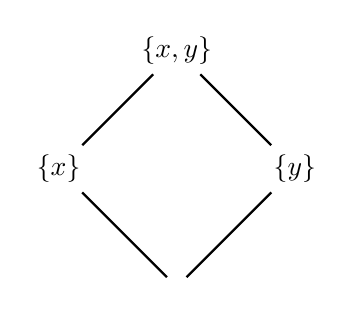
\begin{tikzpicture}[scale=1.5]

  % poset
  \draw (-1cm,0cm) node (v2) {$\{x\}$};
  \draw (1cm,0cm)  node (v3) { $\{y\}$ };
  \draw (0cm,-1cm) node (v4) {$\varnothing$};
  \draw (0cm,1cm)  node (v1) {$\{x,y\}$};

  \draw[thick]  (v1) edge (v2);
  \draw[thick]  (v3) edge (v1);
  \draw[thick]  (v3) edge (v4);
  \draw[thick]  (v2) edge (v4);

  \end{tikzpicture}
\end{center}
\caption{The Hasse Diagram of the poset $(P({x,y}), \subseteq)$.}
\label{fig:hasse}
\end{figure}

A poset can be represented as a hasse diagram, as viewed in figure \ref{fig:hasse}.

\begin{definition}
Let $(W,S)$ be a coxeter system and $T = \{wsw^{-1} | w \in W, s \in S\}$ a set of reflections. $u, w \in W$ define a function $u \to v$ if $l(v) > l(u)$ and $v = ut$ for some $t \in T$.

We define $w \leq v$ if there exist:

\begin{equation}
u \to u_1 \to u_2 \to \dots \to u_k = v
\end{equation}
\end{definition}

A Bruhat order is a partial order on the elements of a Coxeter group. By using the relation defined in the previous definition, we can have a bruhat order as shown in figure \ref{fig:bruhat}.

\begin{figure}
\begin{center}

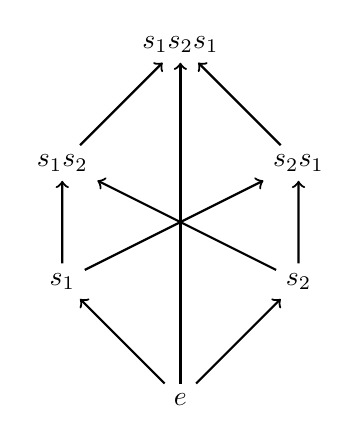
\begin{tikzpicture}[scale=1.5]

  % poset
  \draw (-1cm,0cm) node (v2) {$s_1$};
  \draw (1cm,0cm)  node (v3) {$s_2$ };
  \draw (0cm,-1cm) node (v4) {$e$};
  \draw (-1cm,1cm)  node (v1) {$s_1s_2$};
  \draw (1cm,1cm)  node (v5) {$s_2s_1$};
  \draw (0cm,2cm)  node (v6) {$s_1s_2s_1$};

  \draw[<-, thick]  (v1) edge (v2);
  \draw[->, thick]  (v2) edge (v5);
  \draw[->, thick]  (v3) edge (v1);
  \draw[<-, thick]  (v3) edge (v4);
  \draw[<-, thick]  (v2) edge (v4);
  \draw[->, thick]  (v3) edge (v5);
  \draw[->, thick]  (v1) edge (v6);
  \draw[->, thick]  (v5) edge (v6);
  \draw[->, thick]  (v4) edge (v6);

\end{tikzpicture}
\end{center}
\caption{The Bruhat order $(S_3, \{s_1, s_2\}), T = \{s_1,s_2,s_3,s_4,s_5\}$}
\label{fig:bruhat}
\end{figure}


\begin{theorem}
  Let $u,v \in S_n$, $u \leq v$ if and only if the intersection degree of $u$ is $\leq$ then the one of $v$.
\end{theorem}

\begin{example}
  If we have $35124 \leq 45213$:
  \begin{equation}
    \begin{split}
      3 &\leq 4\\
      35 &\leq 45\\
      135 &\leq 245\\
      1235 &\leq 1245\\
      12345 &\leq 12345
    \end{split}
  \end{equation}
\end{example}

\begin{theorem} [Subword property]
  Let $v = s_1s_2\dotss_q$ reduced word for $v \in W$. Then $u \leq v$ if and only if $u = s_{i_1}s_{i_2} \dots s_{i_k}$ reduced for some $1 \leq i_1 \leq i_2 \leq \dots \leq i_k \leq q$.
\end{theorem}

\begin{proof}
We first prove the \emph{if} part of the theorem. Assume $u \to v$, so $v = ut$ and $l(v) > l(u) = l(utt) = l(vt)$ for some $t \in T$.

By the exchange property:

\begin{equation}
u = vt = s_1s_2\dots \hat{s_i} \dots s_q
\end{equation}

We omit factors iteratively until we have what we want.\\

Second, we prove the \emph{only if} part of the theorem by induction on $l(v) - l(u)$.

If $l(v)-l(u) = 1$ and we have
\begin{equation}
  u = s_1 \dots \hat{s_i} \dots s_q
\end{equation}
with
\begin{equation}
  t = s_q \dots s_i \dots s_q
\end{equation} then $ut = v$ which means that $u \to v$.

If $l(v) - l(u) > 1$ and we have
\begin{equation}
  u = s_1 \dots \hat{s_{a_1}} \dots \hat{s_{a_2}} \dots \hat{s_{a_k}} \dots s_q
\end{equation}
with a minimal $k$ such that $l(v) - l(u) = k$, we take
\begin{equation}
  t = s_q \dots s_{a_k} \dots s_q
\end{equation}
and
\begin{equation}
  ut = s_1 \dots \hat{s_{a_1}} \dots \hat{s_{a_2}} \dots s_{a_k} \dots s_q
\end{equation}


We could have two cases:

\begin{itemize}
  \item Case $l(ut) > l(u)$: \\

  then $l(ut) = l(u) +1$,. so $u \to ut$. $l(v)-l(ut) -1$. By induction $ut \leq v$, so $u \leq v$.

  \item Case $l(ut) < l(u)$: \\

  this will be proved impossible by contradiction. By exchange we have
  \begin{equation}
    ut = s_1 \dots \hat{s_{a_1}} \dots \hat{s_{i}} \dots \hat{s_{a_{k-1}}} \dots s_{a_{k}} \dots s_q
  \end{equation}
  If $i > a_k$ and we have
  \begin{equation}
    t = s_q \dots s_1 \dots s_q
  \end{equation}
then:
  \begin{equation}
    \begin{split}
      vtt &= s_1 \dots s_q (s_q \dots s_{a_k} \dots s_q)(s_q \dots s_i \dots s_q)\\
      &= s_q \dots \hat{s_{a_k}} \dots \hat{s_i} \dots s_q
    \end{split}
  \end{equation}
  which is a contradiction.\\

  If $i < a_k$,
  \begin{equation}
    \begin{split}
      u = utt &= s_1 \dots \hat{s_{a_1}} \dots s_q (s_q \dots \hat{s_{a_k}} \dots s_i \dots \hat{s_k} \dots s_q) (s_q \dots s_{a_k} \dots{s_q})\\
      &= s_1 \dots \hat{s_{a_1}} \dots \hat{s_i} \dots s_{a_k} \dots s_q
    \end{split}
  \end{equation}

  You can see that we omit elements to the left of $a_k$, which contradicts the minimality of $a_k$. This proves that the case when $l(ut) < l(u)$ is impossible. Thus, we have proved the first case true which finishes the proof. \qed

\end{itemize}
\end{proof}

From this theorem we can deduct some corollaries.

\begin{corollary}
  $u \leq v$ if and only if $u^{-1} \leq v^{-1}$.
\end{corollary}

\begin{corollary}
  If $u \leq v$ and $l(v) - l(u) = k$, then
  \begin{equation}
    u \leq u_1 \leq u_2 \leq \dots \leq u_k
  \end{equation}
  with $l(u_i) = l(u) + i$ for every $i$.
\end{corollary}

\begin{proof}
Let $v = s_1 \dots s_q$ and $l(v) = q$, $u \leq v$, $l(v) - l(u) = k$ so $l(u) = q-k$. By subword property

\begin{equation}
  u_1 = s_i \dots \hat{s_{a_k}} \dots s_q = u\underset{t}{\underbrace{s_q \dots s_{a_k} \dots s_q}}
\end{equation}

We have then $l(u_1) = l(ut) = l(u)+1$, so $u \to u_1$ which means that $u \leq u_1$. \qed
\end{proof}

\begin{theorem}[Lifting property]
  If $u, v \in W$ and $s \in S$ with $u \leq w$, $u \leq sw$ and $su \leq w$.
\end{theorem}
\begin{proof}
Take $sw = s_1 \dots s_q$ in a reduced form.

As $sw \leq w$, $w = ss_1\dots s_q$ is also reduced.

As $u \leq w$, $u$ is a subword of $ss_1 \dots s_q$. If $u$ is a subword of $s_1 \dots s_q$, which corresponds to the theorem. If not,
\begin{equation}
  u = ss_{i_1} \dots s_{i_r}
\end{equation}

is reduced with

\begin{equation}
  1 \leq i_1 \leq i_2 \leq \dots \leq i_r \leq q
\end{equation}

So $su = s_{i_1} \dots s_{i_2}$, which is a contradiction as $u \leq su$. The proof of $su \leq w$ is left to the reader. \qed
\end{proof}

\begin{lemma}
  If $u,v \in W$ then it exists a $w \in W$ such that $u \leq w$ and $v \leq w$.
\end{lemma}

\begin{proof}
  We can prove this by induction on $l(u) + l(v)$. Say $l(u) > 0$:

  We take $s \in S$ such that $l(su)= l(u) - 1$. By induction $l(su) + l(v) < l(u) + l(v)$ so it exists indeed a $w \in W$ such that $su \leq w$ and $v \leq w$. We may have two different cases: if $sw \leq w$ or $w \leq sw$:

  \begin{itemize}
    \item Case $w \leq sw$: by the lifting property, $v \leq sw$ and $u \leq sw$.
    \item Case $sw \leq w$: again by the lifting property, $v \leq w$ and $u \leq w$.
  \end{itemize}

  This proves that there exists always an element that respects the lemma, either $w$ or $sw$. \qed
\end{proof}

\begin{corollary}
If $W$ is finite there is an unique maximal $w_0 \in W$.
\end{corollary}

\begin{example}
  In $S_n$ we have $w_0 = n(n-1) \dots 1$.
\end{example}

\begin{corollary}
  If there is a $w_0 \in W$ such that $sw_0 \leq w_0$ for all $s \in S$, then $w \leq w_0$ for all $w \in W$ and $W$ is finite.
\end{corollary}

\begin{proof}
  The proof is left to the reader. You may prove this by induction on $l(w)$, by showing that $w \leq w_0$ for all $w \in W$. Then show finitely many choices of $w$.
\end{proof}

This maximal element is very important because it has some properties that relates it with the set of reflections $T$:

\begin{proposition}
  Let $w_0 \in W$ be the maximal element of $W$ and $T_L(w) = \{t\in T |\  l(tw) < l(w)\}$. The following statements are true:
  \begin{itemize}
    \item $w_0^2 = e$
    \item $l(ww_0) = l(w_0) - l(w)$
    \item $T_L(ww_0) = T \setminus T_L(w_0)$
    \item $l(w_0) = |T|$
  \end{itemize}
\end{proposition}

\begin{corollary}
  $u \leq v$ if and only if $vw_0 \leq uw_0$.
\end{corollary}
